\documentclass[12pt]{article}
\usepackage{float}
\restylefloat{table}
\usepackage{graphicx}
\usepackage{rotating}
\usepackage{color}
\usepackage[dvipsnames]{xcolor}
\usepackage{enumitem}
\usepackage{sidecap}
\usepackage[top=15mm, bottom=15mm, left=15mm, right=15mm]{geometry}
\usepackage{multicol}
\usepackage[dvipsnames]{xcolor}
\usepackage{wrapfig}
\usepackage{hyperref}
\usepackage{courier}


\fboxrule=2pt%border thickness

\pagenumbering{gobble}

\setlength\parindent{0pt}

\begin{document}
\title{DEVILS - Tool for Analysis and Redshifting (TAZ) }


\begin{figure}
\begin{center}
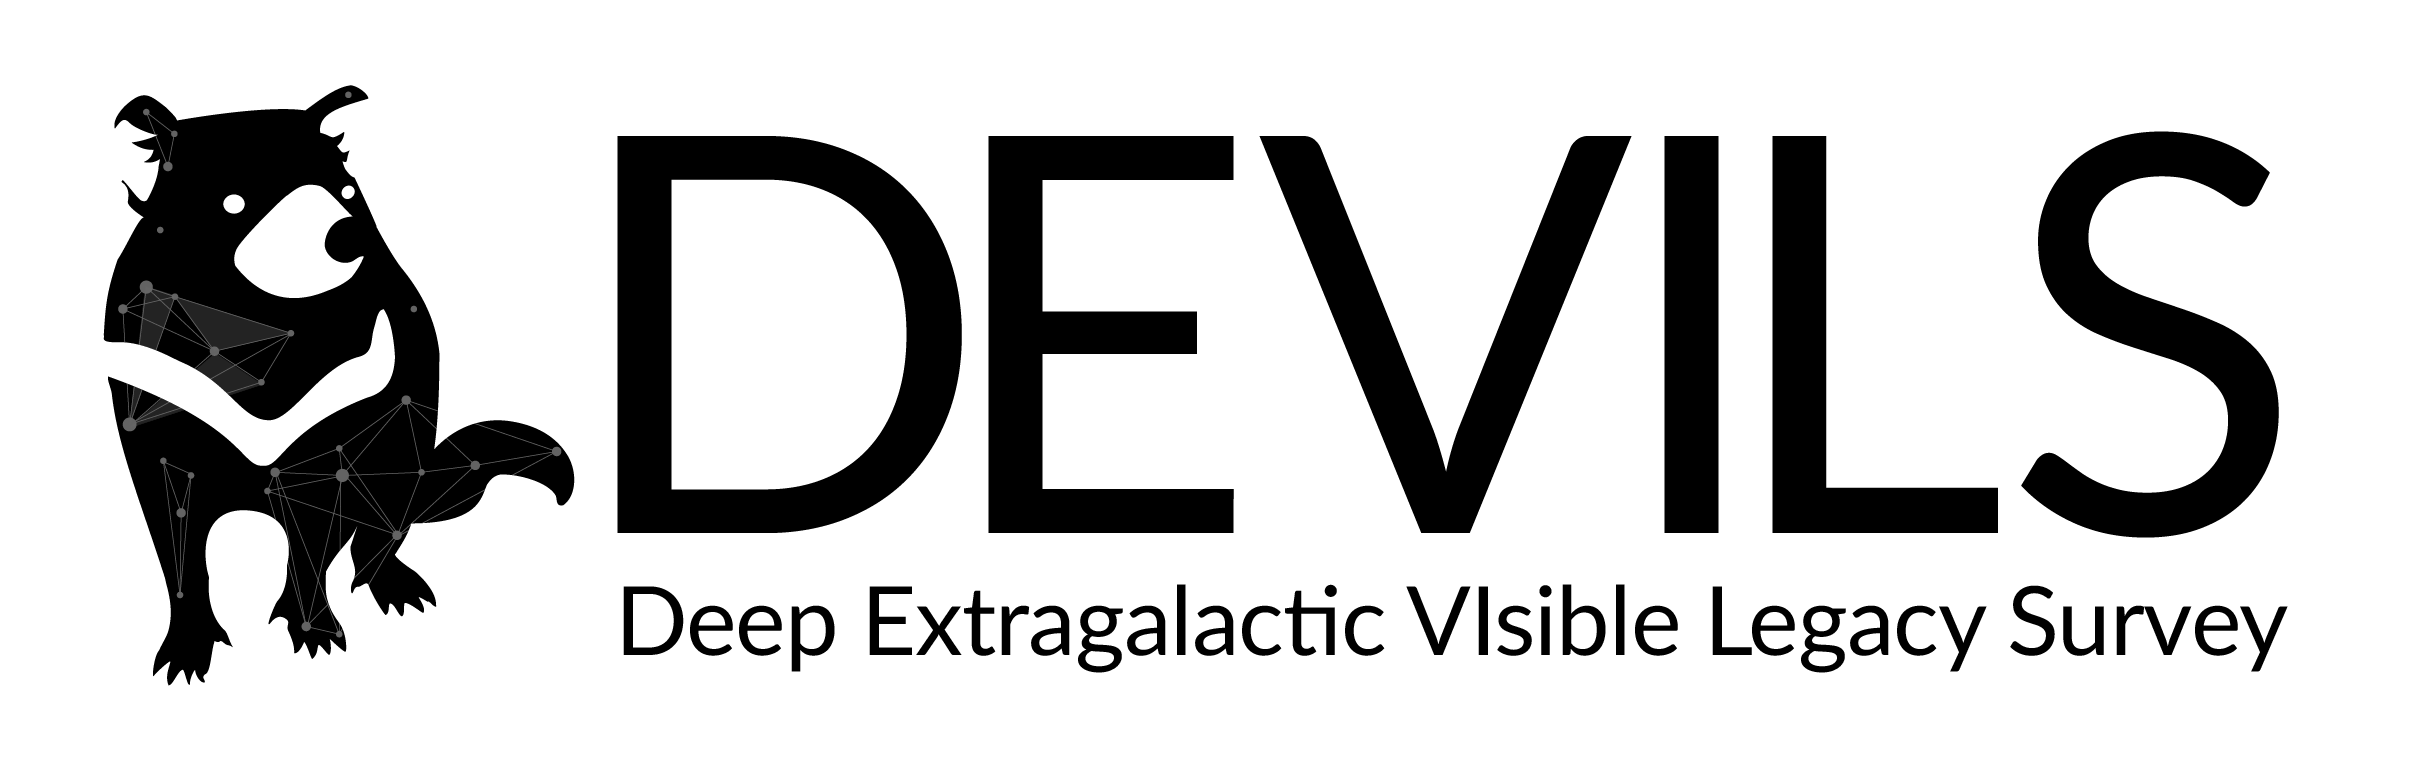
\includegraphics[scale=0.8]{devils-logo_big.png}
\end{center}
\end{figure}

\begin{center}
\Huge {\textcolor{PineGreen}{\textbf{Tool for Analysis and Redshifting (TAZ)}}}
\Huge {\textcolor{PineGreen}{\textbf{ Version 0.1}}}
\end{center}
\normalsize


\section{Installation}

\subsection{External Packages}

There are three main pieces of external software required to run \textsc{taz}. They are i) main coding language \textsc{r}, ii) the 2dfDR data reduction software provided by the the AAO, iii) the AAT targeting/fibre assignment software \textsc{configure}. 

\subsubsection{Installing R}

You can download the version of \textsc{r} specific to your operating systems and via your closest mirror here: \url{https://cran.r-project.org/mirrors.html}. Follow the instructions to install \textsc{r}. You can then check that \textsc{r} is installed correctly, by opening a terminal window and typing: \\


\hspace{10mm} \% R\\

If an \textsc{r} session starts in your terminal you are up and working fine.

\subsubsection{Installing 2dfDR}

The 2dfDR software is used to reduce data from the 2df+AAOmega system at the AAT. Firstly, you can find detailed information regarding the processes in 2dfDR here:  \url{https://www.aao.gov.au/get/document/2dF-AAOmega-obs-manual-69-88.pdf}. In order to install 2dfDR go here: \url{https://www.aao.gov.au/science/software/2dfdr} and download the appropriate version for your operating system. You will then need to follow the installation instructions.

You will then need to set the location of the installed 2dfDR software to your path by add the following (or similar) to your .cshrc/.bashRC/.profile file. For me this is: \\


\hspace{10mm} setenv PATH \$PATH\textbackslash:/Applications/2dfdr-6.46-MacOsX\_ElCapitan/bin \\

For running \textsc{TAZ} we use the command line version of 2dfDR called \textsc{aaorun}. To check this is running correctly, open a terminal and type: \\

\hspace{10mm} \% aaorun help\\

This should display the  \textsc{aaorun} command line options. You can also test the 2dfDR GUI software interface is working, but typing: \\

 
\hspace{10mm} \% drcontrol\\

This should give you a nice image of Saturn and tell you that there are no raw data files in your current directory.

\subsubsection{Installing CONFIGURE}

The AAT uses a piece of software called \textsc{configure} to determine fibre assignments and produce the files required to drive 2df. You can find out about what \textsc{configure} does here: \url{https://www.aao.gov.au/science/software/configure}. On this page follow the online instructions for installing configure.  \\

You will also need to add the path to \textsc{configure}:\\

\hspace{10mm} setenv PATH \$PATH\textbackslash:/Applications/configure-8.4-MacOsX\_ElCapitan\_x86\_64\\

and the environmental variable for \textsc{configure}'s data files:\\

\hspace{10mm}  setenv CONFIG\_FILES /Applications/configure-8.4-MacOsX\_ElCapitan\_x86\_64/data\_files/\\

To your .cshrc, etc.  You can then check that \textsc{configure} is running correctly by opening a terminal and typing: \\

\hspace{10mm} \% configure\\

You should get a pop-up GUI asking which instrument you are using. Don't worry about this, you should not need to do things manually, but \textsc{TAZ} will now be able to call \textsc{configure} to allocate fibres for observing.

\subsection{Installing R packages}

There are a number of R packages that need to be installed. To do this you should just be able to run the \textsc{InstallTAZ.R} script provided. First move to the directory where \textsc{InstallTAZ.R} is located, open an R session in a terminal, using:\\

\hspace{10mm} \% R\\

then run:\\

\hspace{10mm}  \texttt{$>$ source(`InstallTAZ.R')}\\

This will install all of the required packages required to run \textsc{TAZ}. As a quick test type:\\

\hspace{10mm}  \texttt{$>$ installed.packages()}\\

and you should see DEVILSTAZ on this list.

\section{Setting Up the DEVILS Directory Structure}

The first stage in running \textsc{TAZ} is to set up the the DEVILS directory structure. To do this, run the \textsc{setUpDir()} function. This function will create the directory structure including all of the calibrations, IDX files (parameters for 2dfDR), and observability plots/logs for each night you are observing.  To run this structure, you will need to input the run and night range for which you wish to generate the data structure for. First open an R session. Then you will need to load the \textsc{DEVILSTAZ} package (this should be all you need to load whenever you start R):

\hspace{10mm}  \texttt{$>$ library(`DEVILSTAZ')}\\

The \textsc{setUpDir()}  function is then run as:\\

\hspace{10mm}  \texttt{$>$ setUpDir(workingDir=`.', runs=c(`run1\_2017\_12',`run2\_2018\_01'), \$}

\hspace{20mm}   \texttt{dateStart=c(`2017\_12\_18',`2018\_01\_09'),dateEnd=c(`2017\_12\_26',`2018\_01\_22'))}\\

where, \\

 \texttt{workingDir}=directory location you wish to build this structure.\\
 \texttt{runs}=the run names. They must have this format. If you do not know the run you are on, ask Luke (luke.j.davies@uwa.edu.au).\\
 \texttt{dateStart}=First night of each run in year\_month\_day format\\
 \texttt{dateEnd}=Last night of each run in year\_month\_day format\\

Try running this code and explore the directory structure. You can generate this structure for any dates you like. You should something like have:\\

\hspace{5mm} \textbf{data/} 
\vspace{1mm}

\hspace{10mm} \textbf{biases/}
\vspace{1mm}

\hspace{15mm} \textbf{run1\_2017\_12/, ....} 
\vspace{1mm}

\hspace{10mm} \textbf{calibrators/} 
\vspace{1mm}

\hspace{15mm} \textbf{AutoZTemp/} 
\vspace{1mm}

\hspace{15mm} \textbf{filters/} 
\vspace{1mm}

\hspace{15mm} \textbf{GuideStars/}
\vspace{1mm}

\hspace{15mm} \textbf{sensfuncs/}
\vspace{1mm}

\hspace{15mm} \textbf{SkyFibres/}
\vspace{1mm}

\hspace{15mm} \textbf{stdstars/}
\vspace{1mm}

\hspace{10mm} \textbf{darks/} 
\vspace{1mm}

\hspace{15mm} \textbf{run1\_2017\_12/, ....}
\vspace{1mm}

\hspace{10mm} \textbf{idxFiles/} 
\vspace{1mm}

\hspace{10mm} \textbf{logs/} 
\vspace{1mm}

\hspace{10mm} \textbf{observing/} 
\vspace{1mm}

\hspace{15mm} \textbf{D10\_yrPlan2017.png, ....} 
\vspace{1mm}

\hspace{15mm} \textbf{run1\_2017\_12/, ....} 
\vspace{1mm}

\hspace{20mm} \textbf{2017\_12\_18/, ....}
\vspace{1mm}

\hspace{10mm} \textbf{raw/} 
\vspace{1mm}

\hspace{15mm} \textbf{run1\_2017\_12/, ....} 
\vspace{1mm}

\hspace{20mm} \textbf{2017\_12\_18/, ....} 
\vspace{1mm}

\hspace{10mm} \textbf{reduced/}
\vspace{1mm}

\hspace{15mm} \textbf{run1\_2017\_12/, ....} 
\vspace{1mm}

\hspace{20mm} \textbf{2017\_12\_18/, ....} \\

You will populate the \textbf{biases/}, \textbf{darks/}, and \textbf{raw/} part of this structure with the data taken at the AAT, and TAZ will generate reduced data and analysis products in the other parts of the structure.  


\section{Adding Observations}

When observing you will add raw data files to this directory structure. Firstly, at the start of each run, bias and dark frames will be taken. These need to be added to the \textbf{biases/*runName*} and \textbf{darks/*runName*} directories. Note that TAZ will aim to generate a master bias and master dark for all files in this directory, so if there are files that you do not wish to be used in making the master darks/biases please keep them in the  \textbf{biases/*runName*/junk/} or \textbf{darks/*runName*/junk/} sub folders.

Next you will need to place the raw target data under in the relevant directory. This should be easily done as the date in in the file name produced by the AAT. Data for each night observed should be copped to the relevant \textbf{raw/*runName*/*date*}. Once again, TAZ will reduce/analyse all data in this directory. So if there are files you do not wish to be included, add then to the \textbf{raw/*runName*/*date*/junk} folder. You do not need to separate ARC, FLAT and TARGET files in this directory. TAZ will identify and match the correct files based on the configuration used in the FITS header.  

For now, there is is an example small dataset you can get from here \url{https://www.dropbox.com/s/yutdugiwpi4jo3x/TAZRawExample.zip?dl=0}. Once you have this copy the biases, darks and raw data files to your \textbf{biases/}, \textbf{darks/}, and \textbf{raw/} folders under the correct run/date.  

\section{Running TAZ}

Here I will just give a high level overview of running the TAZ software. More detailed descriptions of the individual functions can be accessed via the R help function by simply opening an R terminal and typing: \\

\hspace{10mm}  \texttt{$>$ ?*FUNCTION\_NAME*}\\

In most cases this code will by run end to end with one line. However, here i split it into various sections to explain what the code is doing and to allow the user to run each component separately. 

\subsection{Running the 2dfDR reduction}

First, lets try and run TAZ on our test dataset to just perform the data reduction. To do this, make sure you are in the directory above the \textbf{/data} directory you just generated, and run:

\hspace{10mm} \texttt{$>$ TAZ(user='NewUser', workingDir='.', verbose=2, doReduce=T, doExtract=F, doStack=F, doAutoZ=F, cores=2, doUpdateMaster=F, doTiler=F, zeroPoint=T)}

This should run TAZ over you current directory, reduce the data using 2dfDR. When the code finished, you should find that some of the \textbf{/data/reduced/} sub-folders are populated. Check that this is the case. The most important thing to check is that you have reduced files in the \textbf{/data/reduced/run1\_2017\_12/ \\ 2017\_12\_18/} folder.  If not, go back and check you followed the previous stages correctly, and if you are still experiencing problems contact Luke.  




\subsection{Running the 2dfDR reduction and 1D extraction}

Next we can try and run both a reduction and extract 1D spectra from each of our reduced frames. As TAZ looks for directories that have already been reduced, you will need to delete the products you have previous made in the \textbf{/data/reduced/run1\_2017\_12/2017\_12\_18/} and \textbf{/data/reduced/run1\_2017\_12/ \\ 2017\_12\_19/} directories, before rerunning this code. To do thew reduction and extraction simply set doExtract=T and run:\\

\hspace{10mm} \texttt{$>$ TAZ(user='NewUser', workingDir='.', verbose=2, doReduce=T, doExtract=T, doStack=F, doAutoZ=F, cores=2, doUpdateMaster=F, doTiler=F, zeroPoint=T)}\\

This should run TAZ over you current directory, reduce the data using 2dfDR AND extract 1D spectra. The most important thing to check is that you have individual reduced spectra in the .Rdata format in the \textbf{/data/reduced/allSpec} directory. If not, go back and check you followed the previous stages correctly, and if you are still experiencing problems contact Luke.  \\

As you may not want to re-run the reduction, you can tell TAZ to skip this part. However, you then have to tell it which files to extract 1D spectra from. This is achived by setting  doReduce=F and then adding the variable: toExtractFiles=*a string list of files to extract*. In our example, this would be:\\

 \hspace{10mm} \texttt{$>$ toExtractFiles<-c(`data/reduced/run1\_2017\_12/2017\_12\_18/ \\ 2017\_12\_18\_config\_1\_reduced.fits', `data/reduced/run1\_2017\_12/2017\_12\_19/ \\ 2017\_12\_19\_config\_1\_reduced.fits')}\\
 
  \hspace{10mm} \texttt{$>$ TAZ(user='NewUser', workingDir='.', verbose=2, doReduce=F, doExtract=T, toExtractFiles=toExtractFiles, doStack=F, doAutoZ=F, cores=2, doUpdateMaster=F, doTiler=F, zeroPoint=T)}\\

 This will skip the reduction phase and extract 1D spectra from the reduced files provided.
 
 \subsection{Stacking extracted spectra}
 
 As DEVILS will observe the same spectra over multiple observations, these will need to be stacked to increase single to noise. TAZ can perform this stacking from previously extracted spectra. As TAZ writes all spectra to the \textbf{/data/reduced/allSpec/} directory, the staking procedure simply searches for all instances of a particular ID in this directory and inverse variance weights the spliced spectrum, individual arms and continuum extracted spectra. As we do not wish to extract the spectra again, set \texttt{doExtract=F} and \texttt{doStack=T}. Once again, in order to run this, you must tell TAZ which IDs to stack. This can either be done by providing a vector list of ID (note our example data is from GAMA and all objects are appended with a 'G", in DEVILS this will be 'D'):
 
   \hspace{10mm} \texttt{$>$ toStackIDs<-c(`G006014', 'G006158')}\\
 
  \hspace{10mm} \texttt{$>$ TAZ(user='NewUser', workingDir='.', verbose=2, doReduce=F, doExtract=F, doStack=T,  toStackIDs=toStackIDs, doAutoZ=F, cores=2, doUpdateMaster=F, doTiler=F, zeroPoint=T)}\\ 
  
  A second option is to tell TAZ to try and stack all IDs in the current \textbf{/allSpec} folder. To do this, simply set the \texttt{toStackIDs} value to 'all': \\
  

  \hspace{10mm} \texttt{$>$ TAZ(user='NewUser', workingDir='.', verbose=2, doReduce=F, doExtract=F, doStack=T,  toStackIDs='all', doAutoZ=F, cores=2, doUpdateMaster=F, doTiler=F, zeroPoint=T)}\\   

Run this code now. TAZ should populate the \textbf{/data/reduced/stackedSpec/} folder of your directory structure. 


 \subsection{Running AutoZ on Stacked Spectra}


 \subsection{Updating Master Catalogues with new Redshifts and producing new observing catalogues}


 \subsection{Producing new fibre configuration files}
 
 
 \subsection{Putting it all together}


\section{TAZ inputs list}

\section{TAZ Outputs list}












\textbf{BELOW HERE IS GARBAGE FROM THE OLD VERSION}




\hspace{10mm} \texttt{$>$ TAZ(user=`ldavies',workingDir=`$\sim$/DEVILS/TAZ/',verbose=2, \$ \\
N\_D02A=0,N\_D02B=0, N\_D03=1, N\_D10=1, D02A\_startPlate=0, D02B\_startPlate=0, \$ \\ 
D03\_startPlate=0, D10\_startPlate=0,  doReduce=T, doExtract=T,  \$ \\
toExtractFiles=toExtractFiles, doStack=T, toStackIDs=toStackIDs, doAutoZ=T, \$ \\
toAutoZStacks=toAutoZStacks, doUpdateMaster=T, doTiler=T, \$ \\
DODir=`$\sim$/DEVILS/TAZ/data/observing/run1\_2017\_12/2017\_12\_18/DOCats/')} \\

Below I will briefly explain what each variable in this input means in terms of running the high-level functionality of TAZ:\\

$\bullet$ \texttt{user}=A string identifier which will be added to log files to show who ran the code. \\
$\bullet$ \texttt{workingDir}=The directory location where your previously generated \textbf{data/...} data structure is located.\\
$\bullet$ \texttt{verbose}=How much information to give you about TAZ,  verbose=0,1,2.\\
$\bullet$ \texttt{N\_D?} = Number of new fibre configurations to generate in each field. Use for next night's tiling\\
$\bullet$ \texttt{D?\_startPlate} = Starting plate number for each configuration (either 0 or 1)\\
$\bullet$ \texttt{doReduce} - TRUE/FALSE. Do you want to reduce new data? TAZ will look for new data as files where there is data in the \textbf{raw/} directory for a particular night, but nothing in the corresponding \textbf{reduced/} directory. For the advanced user, you can force this by running \texttt{run2dfDR(toReduce=toReduce)} where \texttt{toReduce} is a list of raw directories you want to reduce. \\
$\bullet$ \texttt{doExtract} - TRUE/FALSE. Do you want to extract 1D spectra from the files you have reduced? If you have set \texttt{doReduce=F} and \texttt{doExtract=T} you will need to provide a list of reduced files to extract..... \\
$\bullet$ \texttt{toExtractFiles} - A string vector list of reduced files for which you wish to extract 1D spectra. Set if \texttt{doReduce=F} and \texttt{doExtract=T}. These need to be the full directory path in the DEVILS data structure. $i.e.$ data/reduced/run2\_2018\_01/2018\_1\_9/2018\_1\_9\_config\_1\_reduced.fits. \\
$\bullet$ \texttt{doStack} - TRUE/FALSE. Do you want to stack extracted spectra? If you have set \texttt{doExtract=F} and \texttt{doStack=T} you will need to provide a list of spectra IDs to stack..... \\
$\bullet$ \texttt{toStackIDs} - A string vector list of ID for which you wish to stack. Here you just provide the IDs in a string. $I.e.$ D10021811.\\
$\bullet$ \texttt{doAutoZ} - TRUE/FALSE. Do you want to run Auto-z over the stacked spectra? If you have set \texttt{doStack=F} and \texttt{doAutoZ=T} you will need to provide a list of stacked spectra files..... \\
$\bullet$ \texttt{toAutoZStacks} - A string vector list of stacked spectra files for which you wish to run Auto-z. These need to be the full directory path in the DEVILS data structure. $i.e.$ data/reduced/stackedSpec/D10021811.Rdata. \\
$\bullet$ \texttt{doUpdateMaster} - TRUE/FALSE. Do you want to update the master catalogue with new redshift. This will produce a new master catalogue with the current date (DMcats). And produce the observing catalogues for the next observation data DOcats. \\ 
$\bullet$ \texttt{doTiler} -  TRUE/FALSE. Do you want to generate new tile configurations for the next night of observations? \\
$\bullet$ \texttt{DODir} - If you have set \texttt{doUpdateMaster=F} and \texttt{doTiler=T} you need to tell the code which observation catalogues to use. Set this to a string with the DOCat directory location. Something like: $\sim$DEVILS/TAZ/data/observing/run1\_2017\_12/2017\_12\_18/DOCats/.\\

For the most common cases you would wish to run something like: \\

\hspace{10mm} \texttt{$>$ TAZ(user=`ldavies',workingDir=`$\sim$/DEVILS/TAZ/',verbose=2, \$ \\
N\_D02A=0,N\_D02B=0, N\_D03=4, N\_D10=4, D02A\_startPlate=0, D02B\_startPlate=0, \$ \\ 
D03\_startPlate=0, D10\_startPlate=0,  doReduce=T, doExtract=T,  \$ \\
doStack=T,  doAutoZ=T, doUpdateMaster=T, doTiler=T )\$ }\\

This will run the code from end to end, finding the new data to reduce, reducing it using 2dfDR, extracting new 1D spectra, stacking new spectra with exisiting spectra, running Auto-z, updating the master catalogue, running the tiling using \textsc{configure}, and producing the new tiling files. 


\subsection{EXAMPLE 1: Manually running 2dfDR using the GUI and extracting spectra, stacking and running AutoZ.}

This will be similar to how the observers at the telescope will use this software, so please see the DEVILS\_Observing\_Manual.pdf for more details. However,  I will briefly describe this process here. 

Once the data has been reduced using 2dFDR (see DEVILS\_Observing\_Manual.pdf), there are certain things that need to be done for any other part of TAZ to be run. Firstly, the reduced files need to be given the correct naming convention and be placed in the correct files in the directory structure.

There must be a reduced file for the full spliced data, the blue arm and the red arm (these will be produced from 2dfDR). These must be named:\\

- Full spliced:  *year*\_*month*\_*day*\_config\_*\#*\_reduced.fits. Where the \# is the number of the configuration taken on that night ($e.g.$ 2017\_12\_18\_config\_4\_reduced.fits)\\
- Blue CCD:  *year*\_*month*\_*day*\_config\_*\#*\_reduced\_blue.fits. Where the \# is the number of the configuration taken on that night ($e.g.$ 2017\_12\_18\_config\_4\_reduced\_blue.fits)\\
- Red CCD:  *year*\_*month*\_*day*\_config\_*\#*\_reduced\_red.fits. Where the \# is the number of the configuration taken on that night ($e.g.$ 2017\_12\_18\_config\_4\_reduced\_red.fits)\\

You must then most these files to the correct part of the directory structure:

- Full spliced: \textbf{data/reduced/*runName*/*year*\_*month*\_*day*/} ($e.g.$ \textbf{data/reduced/run1\_2017\_12/ 2017\_12\_18/}) \\
- Blue CCD: \textbf{data/reduced/*runName*/*year*\_*month*\_*day*/ccd1/} \\
- Red CCD: \textbf{data/reduced/*runName*/*year*\_*month*\_*day*/ccd2/}\\
 
 Once you have done this, you should be able to run TAZ using the following:\\
 
 
 \hspace{10mm} \texttt{$>$ ReducList<-c('data/reduced/run2\_2018\_01/2017\_12\_18\_config\_4\_reduced.fits')}\\
 
 \hspace{10mm} \texttt{$>$ TAZ(user=`ldavies',workingDir=`$\sim$/DEVILS/TAZ/',verbose=2, \$ \\
N\_D02A=0,N\_D02B=0, N\_D03=4, N\_D10=4, D02A\_startPlate=0, D02B\_startPlate=0, \$ \\ 
D03\_startPlate=0, D10\_startPlate=0,  doReduce=F, doExtract=T,  \$ \\
toExtractFiles=ReducList, doStack=T,  doAutoZ=T, doUpdateMaster=T, doTiler=T ) }\\

You only need to give  \texttt{toExtractFiles} the full spliced frame location and it will find the blue and red arms. In this example, only one file is being extracted. However, you can give \texttt{toExtractFiles} a list of files and it will extract all of them. If you only want to extract the spectra and run AutoZ (not update the catalogues/run the tiling), then run: \\

 \hspace{10mm} \texttt{$>$ TAZ(user=`ldavies',workingDir=`$\sim$/DEVILS/TAZ/',verbose=2, \$ \\
N\_D02A=0,N\_D02B=0, N\_D03=4, N\_D10=4, D02A\_startPlate=0, D02B\_startPlate=0, \$ \\ 
D03\_startPlate=0, D10\_startPlate=0,  doReduce=F, doExtract=T,   \$ \\
toExtractFiles=ReducList, doStack=T,  doAutoZ=T, doUpdateMaster=F, doTiler=F ) }\\  
 

\subsection{EXAMPLE 2: Generating new tiling files from an existing catalogue.}

Another thing you may commonly wish to do is generate new tiling files without running any of the reduction/analysis. To do this, you simply need to point TAZ to a specific DOCat directory in the \textbf{data/observing/} part of the data structure. For example:\\

 \hspace{10mm} \texttt{$>$ DODir<-c(`data/observing/run1\_2017\_12/2017\_12\_18/DOCats/')}\\

 \hspace{10mm} \texttt{$>$ TAZ(user=`ldavies',workingDir=`$\sim$/DEVILS/TAZ/',verbose=2, \$ \\
N\_D02A=0,N\_D02B=0, N\_D03=4, N\_D10=4, D02A\_startPlate=0, D02B\_startPlate=0, \$ \\ 
D03\_startPlate=0, D10\_startPlate=0,  doReduce=F, doExtract=F,   \$ \\
 doStack=F,  doAutoZ=F, doUpdateMaster=F, doTiler=T, DODir=DODir) }\\  

This will generate four new configurations for D03 and four for D10 and put them in the data/observing/run1\_2017 \_12/2017\_12\_18/DOCats/Tiling/TileFiles/ directory. 


\section{TAZ Outputs}

TAZ will have generated a large number of output files in different parts of the directory structure. Below is a list of key data products produced by TAZ such that you can easily find things in the data structure: 

\subsection{Raw Data Meta Information:}

\textbf{/data/raw/*runNum*/*date*/*date*\_metaData.Rdata} 

R data file containing meta data from FITS header of all raw files in the current directory. To view this data, move to the directory in which is is contained, open and R session and type: \\

\hspace{10mm}  \texttt{$>$ load(`*date*\_metaData.Rdata')}\\

\hspace{10mm}  \texttt{$>$ metaData}\\
  
 
 This will display the filename, ccd, field, RA/DEC centre, exposure time in seconds, the type of data, fibre configuration, date and grating for each file.  

 
\subsection{Spliced reduced data for each night/configuration:} 
 
 \textbf{/data/reduced/*runName*/*date*/*date*\_config\_?\_reduced.fits} 
 
 FITS file with the fully reduced and spliced data for a particular fibre configuration.

  
\subsection{Blue arm reduced data for each night/configuration:} 
   
   \textbf{/data/reduced/*runName*/*date*/ccd1/*date*\_config\_?\_reduced\_blue.fits} 
   
   FITS file with the fully reduced blue data for a particular fibre configuration.
 
  
\subsection{Red arm reduced data for each night/configuration:} 
  
  \textbf{/data/reduced/*runName*/*date*/ccd2/*date*\_config\_?\_reduced\_blue.fits} 
  
  FITS file with the fully reduced red data for a particular fibre configuration.
 

\subsection{Meta Information for all reduced configurations:} 
 
 \textbf{/data/reduced/*runName*/*date*/*date*\_metaData.Rdata} 
 
 Meta information for all reduced data frames. To view this data, move to the directory in which is is contained, open and R session and type:\\
 

\hspace{10mm}  \texttt{$>$ load(`*date*\_metaData.Rdata')}\\

\hspace{10mm}  \texttt{$>$ metaData}\\

 This will display the filename, ccd, field, RA/DEC centre, exposure time in seconds, the type of data, fibre configuration, date and grating for each file.  
  
 
 \subsection{Flux calibration meta information for each reduced configuration:} 
  
  \textbf{/data/reduced/*runName*/*date*/ccd2/*date*\_config\_?\_reduced\_zeroPoints.Rdata} 
  
  R data file with flux calibration information for each reduced frame. To view this data, move to the directory in which is is contained, open and R session and type:\\
 

\hspace{10mm}  \texttt{$>$ load(`*date*\_config\_?\_reduced\_zeroPoints.Rdata')}\\

\hspace{10mm}  \texttt{$>$ zeroPoints}\\

This will display:\\

ZP - Magnitude zero point of the frame calculated from standard stars     \\
ZPMAD - Median average deviation of ZP    \\
ZPRMS - RMS of ZP   \\
ZPNUM - Number of standards used to calculate ZP\\
FLUXSC - The flux scaling to convert counts to ergs/sec/cm$^2$/Ang/\\
ZP\_red... - Same values for red and blue arm data individually.  \\


 \subsection{Individual extracted spectra from corresponding reduced configuration/night:}
 
   \textbf{/data/reduced/*runName*/*date*/ccd2/*date*\_config\_?\_reduced\_spec/}
   
  Directory containing all individually reduced spectra from the corresponding  configuration. This directory will also contain 1D plots if requested in TAZ. Each spectrum is stored as an R data structure. To view this data, move to the directory in which is is contained, open and R session and type (for example):\\
  
\hspace{10mm}  \texttt{$>$ load(`2017\_12\_18\_G2271755.Rdata')}\\

\hspace{10mm}  \texttt{$>$ spec}\\  

This structure contains various data and meta information for this observation, such a flux, wavelength, sky. It also retains the individual blue and red arms of the spectrum prior to splicing. Note that these are not flux calibrated, but contain the flux calibration information to convert pixels to ergs/sec/cm$^2$/A (fluxSc). To view the spectrum simply type:\\

 \hspace{10mm}  \texttt{$>$ magplot(spec\$wave, spec\$flux, type='l')}\\  



 \subsection{Individual spectra meta information for each configuration/night:} 
 
  \textbf{/data/reduced/*runName*/*date*/ccd2/*date*\_config\_?\_reduced\_meta.Rdata} 
  
  R data file containing the meta information for each spectrum row in the corresponding reduced file. To view this data, move to the directory in which is is contained, open and R session and type:\\
 

\hspace{10mm}  \texttt{$>$ load(`*date*\_config\_?\_reduced\_meta.Rdata')}\\

\hspace{10mm}  \texttt{$>$ meta}\\

This will display:\\

ID - Source ID from input catalogue    \\
RA - Fibre RA \\
DEC - Fibre DEC \\
X - Fibre X \\
Y - Fibre Y \\
XERR - Fibre X error \\
YERR- Fibre Y error\\
THETA - Fibre angle \\
TYPE - Type of source (Target, sky, standard, guide)\\
MAG - Magnitude of source from input cat\\
FIBRE - Fibre Number\\
 
 
 
 
 \section{TAZ data flow and components}
  

\end{document}

